\chapter{Effective Spin Hamiltonian}

In this chapter we will start with a Hamiltonian

\begin{equation}
\label{Ham1}
\hat{H} = \sum_{i=1}^{N_e} \hat{H}^{(1)}(\textbf{r}_i) + \frac{1}{2} \sum_{\substack{i,j = 1 \\ i \neq j}} ^ {N_e} v(\textbf{r}_i - \textbf{r}_j)
\end{equation}

where $v$ is the electron-electron interaction and where $\hat{H}^{(1)}$ is the single particle Hamiltonian:

\begin{equation}
\hat{H}^{(1)}(\textbf{r}) = -\frac{\hbar^2}{2m}\nabla^2_{\textbf{r}} + \text{U}(\textbf{r}) + \lambda\bs{\sigma}\bs{\nabla}V(\textbf{r}) \times \textbf{p}
\end{equation}

Where $\lambda = \frac{\hbar^2}{4m^2c^2}$ is the spin orbit coupling constant and $\text{U}(\bs{r})$ is a periodic potential. The second quantized form of this Hamiltonian can be approximated by a version of the Hubbard model. The original Hubbard model, was developed to describe the single-band magnetism \cite{Hubbard1963}, it also describes the transition between conducting and insulating systems, predicting the existence of Mott insulators, materials which should be conducting according to band theory, but they are insulating due to electron-electron interactions.

We will consider a half filled system in the strong coupling limit. Ignoring electron hopping and spin orbit interaction, the ground state of this system is massively degenerated. We will find an effective Hamiltonian considering that the hopping term and the spin interaction term act on this subspace. This effective Hamiltonian will be the sum of three spin interactions: an exchange interaction $J\bs{S}_i\bs{S}_j$ with $J>0$, a Dzyaloshinkii-Moriya interaction $\bs{D}\bs{S}_i\times\bs{S}_j$ and an anisotropic interaction $\bs{S}_i \bs{\Gamma} \bs{S}_j$ known as pseudodipolar interaction \cite{Moriya1960}.

\begin{section}{Single particle in a periodic potential}

First we will define a suitable basis for the single particle wavefunctions. To do so, we will consider the single particle Hamiltonian without the spin orbit interaction term:

\begin{equation}
\label{LaticeHam}
\hat{H}^{(1)}_{\text{NSOI}}(\textbf{r}) = -\frac{\hbar^2}{2m}\nabla^2_{\textbf{r}} + \text{U}(\textbf{r})
\end{equation}

Where $\text{U}(\textbf{r})$ has the symmetry of the lattice, i.e. $\text{U}(\textbf{r} + \textbf{R}) = \text{U}(\textbf{r})$ for all Bravais lattice vectors $\textbf{R}$(\ref{AP1A}). Let $\hat{H}^{(1)}_{\text{NSOI}}$ act on a Hilbert space $\mathcal{H}$ and let $\ket{\phi} \in \mathcal{H}$, then, the group of translation symmetries defined by $\bra{\bs{r}} T_{\textbf{R}} \ket{\phi} = \bra{\bs{r} + \bs{R}} \ket{\phi}$ is an abelian group, therefore its irreducible representations are one-dimensional, that is, within an energy level $n$ the wavefunctions of that level transform according to the representation they belong. If $\Gamma^{\textbf{k}}$ is a one dimensional representation and $\ket{\phi_n, \bs{k}}$ is a wavefunction in the energy level $n$ belonging to that representation then $T_{\textbf{R}}\ket{\phi_{n, \textbf{k}}} = \Gamma^{\textbf{k}}(\textbf{R}) \ket{\phi_{n, \textbf{k}}}$. Now, imposing periodic boundary conditions, $\Gamma^{\textbf{k}}(\textbf{a}_\mu)^{L_\mu} = 1$, where $\bs{a}_\mu$ are the primitive translations and $L_\mu$ is the number of lattice sites in the $\mu$ direction as defined in \ref{AP1A}. This can be accomplished if we label the representation with a vector of the first Brillouin zone and have $\Gamma^{\textbf{k}}(R) = e^{i \textbf{k} \textbf{R}}$. Therefore, for a wavefunction in a periodic lattice we have:

\begin{equation}
\label{Bloch1}
\bra{\bs{r}+\bs{R}} \ket{\phi_{n, \textbf{k}}} = e^{i\textbf{k}\textbf{R}}\bra{\bs{r}} \ket{\phi_{n, \textbf{k}}}
\end{equation}

Which is the well-known Bloch function form. Here, $n$ is called the band index, and $\textbf{k}$ is the quasimomentum. The energy of this wavefunction is $\epsilon_{n \textbf{k}}$.  Notice that both $\phi_{n,\textbf{k}}$ and $\epsilon_{n \textbf{k}}$ are periodic functions of $\textbf{k}$ in the reciprocal lattice.

The Bloch function is extended over the whole crystal volume $V$. We would like to work with a localized basis. An alternative orthonormal basis are the Wannier functions $\ket{\psi_{in}}$, defined in terms of the Bloch functions as:

\begin{align}
\bra{\bs{r}}\ket{\phi_{n\bs{k}}} &= \frac{1}{\sqrt{M}}\sum_{\bs{R}} e^{i\bs{k}\bs{R}} \bra{\bs{r}}\ket{\psi_{\bs{R}n}}  \label{Wannier1} \\
\bra{\bs{r}}\ket{\psi_{in}} &= \frac{1}{\sqrt{M}} \sum_{\bs{k}\in BZ} e^{-i\textbf{k}\textbf{R}_i} \bra{\bs{r}}\ket{\phi_{n\bs{k}}}\label{Wannier2}
\end{align}

Where $M$ is the number of lattice sites as defined in \ref{AP1A}. Using \ref{Bloch1} we see that $\psi_{in}(\textbf{r}) = \psi_{0n}(\textbf{r}-\textbf{r}_i) \equiv \psi_{n}(\textbf{r}-\textbf{r}_i)$, so we only need to define one Wannier function for each band and the others are obtained by translations. From now on we will restrict ourselves to a fixed band, so we will drop the band index. Additionally, we will include the spin state, therefore the basis states will have two quantum numbers one for the site and one for the spin state. We will adopt the notation $\ket{i\sigma}$ for the basis state of site $i$ with spin state $\sigma = \uparrow, \downarrow$, or just $\ket{i}$ when the spin state is irrelevant. Fock space states with small number of particles will be denoted as $\ket{i\sigma, j\sigma'}$, for a state with a particle at site $i$ with spin $\sigma$ and a particle at $j$ with spin $\sigma'$, or $\ket{ij}$ when spin is irrelevant.

\end{section}

\begin{section}{Derivation of the single-band Hubbard model}

In this section we will derive the second quantized form of \ref{Ham1} using the Wannier function basis. Let $\hat{c}_{j \sigma}^\dagger$ and $\hat{c}_{j \sigma}$ create and annihilate a particle in the state $\ket{j\sigma}$. In this basis, the second quantized form of \ref{Ham1} is:

\begin{equation}
\hat{H} = \sum_{i,j,\sigma, \sigma'} \bra{i\sigma} \hat{H}^{(1)} \ket{j\sigma'} \hat{c}_{i \sigma}^\dagger \hat{c}_{j \sigma'} + \frac{1}{2} \sum_{i,j,k,l, \sigma, \sigma'} \bra{ij} \hat{v} \ket{kl} \hat{c}_{i \sigma}^\dagger \hat{c}_{j \sigma'}^\dagger \hat{c}_{l \sigma'} \hat{c}_{k \sigma}
\end{equation}

Where we assumed $\hat{v}$ to be spin independent. This can be rewritten as:

\begin{equation}
\hat{H} = -\sum_{i,j,\sigma, \sigma'} (\delta_{\sigma, \sigma'} t_{ij} + \boldsymbol{\Delta}_{ij} \boldsymbol{\sigma}_{\sigma, \sigma'}) \hat{c}_{i \sigma}^\dagger \hat{c}_{j \sigma'} + \frac{1}{2} \sum_{i,j,k,l, \sigma, \sigma'} \bra{ij} \hat{v} \ket{kl} \hat{c}_{i \sigma}^\dagger \hat{c}_{j \sigma'}^\dagger \hat{c}_{l \sigma'} \hat{c}_{k \sigma}
\end{equation}

Where $t_{ij} = -\bra{i} -\frac{\hbar^2}{2m}\nabla^2_{\textbf{r}} + \text{U}(\textbf{r}) \ket{j}$ and $\boldsymbol{\Delta}_{ij} = -\bra{i} \lambda \boldsymbol{\nabla}V(\textbf{r}) \times \textbf{p} \ket{j}$. Notice that $\bs{\Delta}_{ij} = - \bs{\Delta}_{ji}$, for example, in the $x$ component:

\begin{align*}
\Delta_{ij,x} &= -\bra{i} \lambda (\partial_y V(\bs{r}) p_z - \partial_z V(\bs{r}) p_y) \ket{j} = i \hbar \lambda \int d \bs{r} \phi_i(\bs{r})^* (\partial_y V(\bs{r}) \partial_z - \partial_z V(\bs{r}) \partial_y) \phi_j(\bs{r}) = \\
&= -i\hbar\lambda \int d\bs{r} \left[ \partial_z(\phi_i(\bs{r})^*\partial_y V(\bs{r}) - \partial_y(\phi_i(\bs{r})^*\partial_z V(\bs{r}) \right] \phi_j(\bs{r}) = \\
&= -i\hbar\lambda \int d\bs{r} \left[ \partial_z \phi_i(\bs{r})^* \partial_y V(\bs{r}) - \partial_y \phi_i(\bs{r})^*\partial_z V(\bs{r}) \right] \phi_j(\bs{r}) = \\
&= \int d\bs{r} \phi_j(\bs{r}) \lambda (\bs{\nabla}V(\bs{r}) \times \bs{p})_x \phi_i(\bs{r})^* = - \Delta_{ji,x}
\end{align*}

Therefore $\bs{\Delta}_{ii} = 0$. Notice also that $\bs{\Delta}_{ij}$ is purely imaginary.
We can impose that $t_{ii} = t(0) = 0$. For a system of strongly correlated electrons we can assume that:

\begin{itemize}
\item A property of the Wannier functions $\Phi_j$ is that they have exponentially decreasing overlaps, therefore $t_{ij}$ and $\boldsymbol{\Delta}_{ij}$ will decay rapidly with the distance $|\textbf{r}_i-\textbf{r}_j|$. In an isotropic system we can approximate:

\begin{equation}
t_{ij} = \begin{cases}
             t,  & \text{for } (i,j) \text{ nearest neighbous} \\
             0,  & \text{otherwise}
       \end{cases} \quad
\end{equation}

and

\begin{equation}
\bs{\Delta}_{ij} = \begin{cases}
             \bs{\Delta}_{ij},  & \text{for } (i,j) \text{ nearest neighbours} \\
             0,  & \text{otherwise}
       \end{cases} \quad
\end{equation}

Hubbard models with hopping terms further than nearest neighbors are also interesting and will be considered in next chapter.  

\item Taking into account the locality of the Wannier functions and the Coulomb interaction, the dominant contribution of $\bra{ij} \hat{v} \ket{kl}$ will come from $i=j=k=l$. Terms with $i=k$ and $j=l$ also contribute when $i, j$ are nearest neighbours. Therefore we approximate:

\begin{equation}
\bra{ij} \hat{v} \ket{kl} =
	\begin{cases}
		\text{U}, & \text{if } i=j=k=l \\
		\text{V}, & \text{if } i=k \text{ and } j=l \text{ where } (i,j) \text{ nearest neighbours} \\
		0, & \text{otherwise}
	\end{cases}						
\end{equation}

Where we defined:

\begin{align}
\text{U} &= \frac{1}{2} \int d\bs{r} d\bs{r}' \phi(\bs{r})^* \phi(\bs{r}')^* \hat{v}(\bs{r}-\bs{r}') \phi(\bs{r}') \phi(\bs{r}) \\
\text{V} &= \int d\bs{r} d\bs{r}' \phi(\bs{r})^* \phi(\bs{r}'-\bs{R}_1)^* \hat{v}(\bs{r}-\bs{r}') \phi(\bs{r}'-\bs{R}_1) \phi(\bs{r})
\end{align}

Where $\phi(\bs{r})$ is the Wannier function centered at the origin and $\bs{R}_1$ is a nearest neighbour lattice vector. Notice that we made explicit use of the translational invariance of the system. Also, for $i=j=k=l$ the Pauli principle requires $\sigma' = -\sigma$.

\end{itemize}

Taking these approximations and writing $\hat{c}_{i \sigma}^\dagger \hat{c}_{j \sigma'}^\dagger \hat{c}_{j \sigma'} \hat{c}_{i \sigma} = \hat{n}_{i \sigma} \hat{n}_{j \sigma'}$, we obtain:

\begin{equation}
\label{HubbardWithNonLocalInt}
\hat{H} = -\sum_{\langle i,j \rangle, \sigma, \sigma'}(\delta_{\sigma, \sigma'} t_{ij} + \bs{\Delta}_{ij} \bs{\sigma}_{\sigma, \sigma'})\hat{c}_{i \sigma}^\dagger \hat{c}_{j \sigma'} + \text{U} \sum_{i=1}^M \hat{n}_{i\uparrow}\hat{n}_{i\downarrow} + \text{V} \sum_{i,j,\sigma,\sigma'}  \hat{n}_{i \sigma} \hat{n}_{j \sigma'}
\end{equation}

Now, in a half filling system this Hamiltonian can be well approximated by an effective Hamiltonian without non local Coulomb interactions:

\begin{equation}
\label{Intermediate}
\hat{H} = -\sum_{\langle i,j \rangle, \sigma, \sigma'}(\delta_{\sigma, \sigma'} t_{ij} + \bs{\Delta}_{ij} \bs{\sigma}_{\sigma, \sigma'})\hat{c}_{i \sigma}^\dagger \hat{c}_{j \sigma'} + \text{U}^* \sum_{i=1}^M \hat{n}_{i\uparrow}\hat{n}_{i\downarrow}
\end{equation}

Where $\text{U}^* = \text{U} - \text{V}$. The physical reason for this is that the energy difference when the Coulomb interaction pushes an electron from a double occupied site to an empty site is $\text{U}-\text{V}$ in \ref{HubbardWithNonLocalInt}, because the number of double occupied sites is reduced by one but the number of adjacent occupied sites is increased by one. This is illustred in Figure \ref{Fig2.1}. A more rigouros derivation of this effective model can be found in \cite{Schuler2013}. Altough $\text{V} < \text{U}$, they can be comparable in magnitude, and $\text{U}^*$ can be reduced by a factor of $0.5$ or more.

\begin{figure}
\centering
  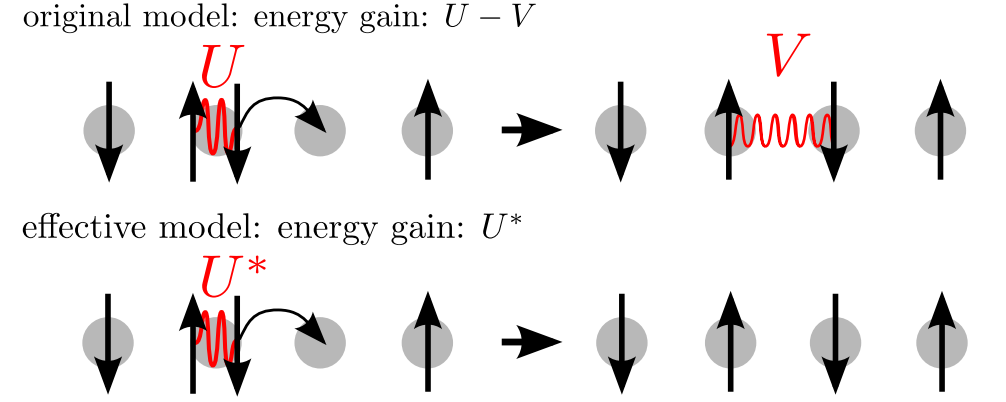
\includegraphics[width=0.5\linewidth]{../Figures/non_local_coulomb.png}
  \caption{Image from \cite{Schuler2013}. In a half-filled system decreasing the number of double occupancies increases the number of adjacent occupied sites, and so the energy difference is reduced to $\text{U}-\text{V}$.} 
\label{Fig2.1}
\end{figure}

Now, abusing the notation and writing $\text{U} = \text{U}^*$ we arrive at the model that we will use in the next sections:

\begin{equation}
\label{Hubbard}
\hat{H} = -\sum_{\langle i,j \rangle, \sigma, \sigma'}(\delta_{\sigma, \sigma'} t_{ij} + \bs{\Delta}_{ij} \bs{\sigma}_{\sigma, \sigma'})\hat{c}_{i \sigma}^\dagger \hat{c}_{j \sigma'} + \text{U} \sum_{i=1}^M \hat{n}_{i\uparrow}\hat{n}_{i\downarrow}
\end{equation}

\begin{subsection}{Hubbard model}

In the absence of spin-orbit interaction the model \ref{Hubbard} becomes the well-known Hubbard model: $\hat{H} = -\sum_{\langle i,j \rangle, \sigma} t_{ij} \hat{c}_{i \sigma}^\dagger \hat{c}_{j \sigma} + \text{U} \sum_{i=1}^M \hat{n}_{i\uparrow}\hat{n}_{i\downarrow}$. This model has been extensively studied since its proposal in 1963 by Hubbard \cite{Hubbard1963}. Despite its simplicity the ground state has no analytic form in more than one dimensions, and different computational methods must be used to study it. Originally the Hubbard model was proposed to describe electron correlations in $d$ or $f$ bands in transition metals. The result was a simplified model to predict metal-insulator transitions. However, it exhibits much richer phenomena. It can be considered an impoved tight binding model, describing Mott insulators, which cannot be describied by band theory (i.e. they should be conductors according to band theory, but electron-electron interactions keep away from). Also, the attractive Hubbard model (where $\text{U} < 0$) can be considered an effective model relevant for understanding high temperature superconductivity \cite{Alexandrov1981}.

\end{subsection}

\end{section}

\begin{section}{Effective Hamiltonian for half-filling system}

At half filling, in the $t << \text{U}$ limit, which correspond to the strong coupling limit, we can apply perturbation theory to obtain the Heisenberg model from the Hubbard Hamiltonian \ref{Hubbard}. First notice that in the case $t = 0$ the ground state corresponds to having all sites single-occupied. There are two possible spin orientations for each sites, so there is a $2^M$ degeneracy. The ground state energy is $0$. The first exited states are obtained by moving one electron from one site to another, thus leaving one empty site and one double-occupied site. The energy of one of these states is $\text{U}$. Now, if we turn the kinetic term on as a perturbation, having two neighbors electrons with antiparallel spin will allow them to hop and reduce the kinetic energy, whereas while being parallel this hopping is not allowed and there is no energy reduction. Therefore, we can see that when turning the kinetic term on antiparallel alignment will be favored. 

Let us write $\hat{H} = \hat{H}_0 + \hat{H}_t$, where $\hat{H}_0$ is the Hamiltonian for $t=0$ i.e. $\hat{H}_0 = \text{U} \sum_{i=1}^M \hat{n}_{i\uparrow}\hat{n}_{i\downarrow}$ and $\hat{H_t} = -\sum_{\langle i,j \rangle, \sigma, \sigma'}(\delta_{\sigma, \sigma'} t + \bs{\Delta}_{ij} \bs{\sigma}_{\sigma, \sigma'})\hat{c}_{i \sigma}^\dagger \hat{c}_{j \sigma'}$. Let $\ket{\phi}$ and $\ket{\phi'}$ be states from the ground state of $\hat{H}_0$, then we know $\bra{\phi'} \hat{H_0} \ket{\phi} = 0$ and in first order in $t$ $\bra{\phi'} \hat{H} \ket{\phi} = \bra{\phi'} \hat{H_t} \ket{\phi} = 0$ since $\hat{c}_{i \sigma}^\dagger \hat{c}_{j \sigma}$ moves an electron from site $j$ to $i$ thus leaving $i$ doubly occupied, therefore $\hat{H_t} \ket{\phi}$ has no superposition with $\phi'$. In second order we have:

\begin{equation}
\bra{\phi'} \hat{H} \ket{\phi} = \sum_s \frac{\bra{\phi'} \hat{H_t} \ket{s}\bra{s} \hat{H_t} \ket{\phi}}{E_0-E_s}
\end{equation}

The sum being over all excited states. Since $\hat{H_t}\ket{\phi}$ is a superposition of states with exactly one double occupied site and one empty site, we see that only excited states with one double occupied site will contribute. These states have energy $E_s = \text{U}$ therefore we have $\bra{\phi'} \hat{H} \ket{\phi} = -\frac{1}{\text{U}}\sum_s \bra{\phi'} \hat{H_t} \ket{s}\bra{s} \hat{H_t} \ket{\phi} = \bra{\phi'} -\frac{\hat{H_t^2}}{\text{U}} \ket{\phi}$. These means that within the subspace generated by the ground states of $\hat{H_0}$, $\hat{H}$ acts as an effective Hamiltonian $\hat{H}_{\text{eff}} = -\frac{\hat{H_t^2}}{\text{U}}$. Now,

\begin{align}
\label{PertNoEMF}
&\bra{\phi'} -\frac{\hat{H_t^2}}{\text{U}} \ket{\phi} = \nonumber \\
&= -\frac{1}{\text{U}} \bra{\phi'}\sum_{\langle i,j \rangle, \sigma_1, \sigma_2} \sum_{\langle i',j' \rangle, 					\sigma_3, \sigma_4} \left( \delta_{\sigma_1, \sigma_2} t + \bs{\Delta}_{ij} \bs{\sigma}_{\sigma_1, \sigma_2} \right) \left( \delta_{\sigma_3, \sigma_4} t + \bs{\Delta}_{i'j'} \bs{\sigma}_{\sigma_3, \sigma_4} \right)\hat{c}_{i\sigma_1}^\dagger \hat{c}_{j \sigma_2} \hat{c}_{i' \sigma_3}^\dagger \hat{c}_{j'\sigma_4} \ket{\phi} = \nonumber \\
&= -\frac{1}{\text{U}} \bra{\phi'}\sum_{\langle i,j \rangle, \sigma_1, \sigma_2, \sigma_3, \sigma_4} \left( \delta_{\sigma_1, \sigma_2} t + \bs{\Delta}_{ij} \bs{\sigma}_{\sigma_1, \sigma_2} \right) \left( \delta_{\sigma_3, \sigma_4} t - \bs{\Delta}_{ij} \bs{\sigma}_{\sigma_3, \sigma_4} \right)\hat{c}_{i\sigma_1}^\dagger \hat{c}_{j \sigma_2} \hat{c}_{j \sigma_3}^\dagger \hat{c}_{i\sigma_4} \ket{\phi} = \nonumber \\
&-\frac{1}{\text{U}} \bra{\phi'} \sum_{\langle i,j \rangle, \sigma_1, \sigma_2, \sigma_3, \sigma_4} (t^2 						\delta_{\sigma_1 \sigma_2}\delta_{\sigma_3 \sigma_4} + t\bs{\Delta}_{ij}(\delta_{\sigma_3 \sigma_4}			\bs{\sigma}_{\sigma_1 \sigma_2} - \delta_{\sigma_1 \sigma_2} \bs{\sigma}_{\sigma_3 \sigma_4}) - (\bs{\Delta}_{ij}\bs{\sigma}_{\sigma_1 \sigma_2})(\bs{\Delta}_{ij} \bs{\sigma}_{\sigma_3 \sigma_4}) ) \hat{c}_{i\sigma_1}^\dagger \hat{c}_{i\sigma_4} \hat{c}_{j 		\sigma_2} \hat{c}_{j \sigma_3}^\dagger \ket{\phi} = \nonumber \\
& \bra{\phi'} \hat{H}_J + \hat{H}_D + \hat{H}_P \ket{\phi}
\end{align}

In the second line we imposed $i=j'$ and $j=i'$ since that's the only way $\hat{H_t^2}\ket{\phi}$ has no double occupied sites and so the matrix element does not vanish. We also used $\bs{\Delta}_{ij} = - \bs{\Delta}_{ji}$. We defined:

\begin{align}
\hat{H}_J &= -\frac{t^2}{\text{U}} \sum_{\langle i,j \rangle, \sigma, \sigma'} \hat{c}_{i\sigma}^\dagger \hat{c}_{i\sigma'} \hat{c}_{j\sigma} \hat{c}_{j \sigma'}^\dagger \\
\hat{H}_D &= -\frac{t}{\text{U}}\sum_{\langle i,j \rangle, \sigma_1, \sigma_2, \sigma_3, \sigma_4} \bs{\Delta}_{ij}(\delta_{\sigma_3 \sigma_4}	\bs{\sigma}_{\sigma_1 \sigma_2} - \delta_{\sigma_1 \sigma_2} \bs{\sigma}_{\sigma_3 	\sigma_4}) \hat{c}_{i\sigma_1}^\dagger \hat{c}_{i\sigma_4} \hat{c}_{j \sigma_2} \hat{c}_{j \sigma_3}^\dagger \\
\hat{H}_P &= \frac{1}{\text{U}}\sum_{\langle i,j \rangle, \sigma_1, \sigma_2, \sigma_3, \sigma_4} (\bs{\Delta}_{ij}\bs{\sigma}_{\sigma_1 \sigma_2})(\bs{\Delta}_{ij} \bs{\sigma}_{\sigma_3 \sigma_4}) \hat{c}_{i\sigma_1}^\dagger \hat{c}_{i\sigma_4} \hat{c}_{j \sigma_2} \hat{c}_{j \sigma_3}^\dagger
\end{align}

Let us now introduce the on-site spin operators:

\begin{equation}
\label{SpinOperators}
\boldsymbol{S}_i = \frac{1}{2} \sum_{\sigma, \sigma'} \hat{c}_{i \sigma}^\dagger \boldsymbol{\sigma}_{\sigma, \sigma'} \hat{c}_{i \sigma'}
\end{equation}

Which satisfy:

\begin{align}
\hat{c}_{i \sigma}^\dagger \hat{c}_{i \sigma'} &= \delta_{\sigma \sigma'} \frac{1}{2} (n_{i \uparrow} + n_{i \downarrow}) + \boldsymbol{S}_i\boldsymbol{\sigma}_{\sigma', \sigma} \label{SpinOperatorInv1}\\ 
\hat{c}_{i \sigma} \hat{c}_{i \sigma'}^\dagger &= \delta_{\sigma \sigma'} \frac{1}{2} (2 - n_{i \uparrow} - n_{i \downarrow}) - \boldsymbol{S}_i\boldsymbol{\sigma}_{\sigma, \sigma'} \label{SpinOperatorInv2}
\end{align}

In the half-filling case we have $n_{i \uparrow} + n_{i \downarrow} = 1$ and we can show two important relations. First:

\begin{align*}
&\sum_{\sigma \sigma'} \left(\frac{1}{2}\delta_{\sigma \sigma'} + \boldsymbol{S}_i\boldsymbol{\sigma}_{\sigma' \sigma}\right)\left(\frac{1}{2}\delta_{\sigma \sigma'}-\boldsymbol{S}_j\boldsymbol{\sigma}_{\sigma \sigma'}\right) = \sum_{\sigma \sigma'} \left\{ \frac{1}{4}\delta_{\sigma \sigma'} - \sum_{ab} S_i^aS_j^b 	\boldsymbol{\sigma}_{\sigma'\sigma}^a \boldsymbol{\sigma}_{\sigma \sigma'}^b \right\}= \\
&= \frac{1}{2} - \sum_{ab} S_i^aS_j^b	2\delta_{ab} = \frac{1}{2} - 2\boldsymbol{S}_i\boldsymbol{S}_j
\end{align*}

Where we have neglected the term $\sum_{\sigma \sigma'} \frac{1}{2}\delta_{\sigma,\sigma'}(\bs{S}_i\bs{\sigma}_{\sigma',\sigma} - \bs{S}_j\bs{\sigma}_{\sigma,\sigma'})$ because eventually we will sum over all $\langle i, j \rangle$ and it will cancel out. We also used the well known property $tr(\bs{\sigma}^a\bs{\sigma}^b)=2\delta_{a,b}$. And second:

\begin{align*}
&\sum_{\sigma_1, \sigma_2, \sigma_3, \sigma_4}\boldsymbol{\Delta}_{ij}(\delta_{\sigma_3 \sigma_4}\boldsymbol{\sigma}_{\sigma_1 \sigma_2} - \delta_{\sigma_1 \sigma_2} \boldsymbol{\sigma}_{\sigma_3\sigma_4})\left(\frac{1}{2}\delta_{\sigma_1 \sigma_4} + \bs{S}_i\bs{\sigma}_{\sigma_4 \sigma_1}\right)\left(\frac{1}{2}\delta_{\sigma_2 \sigma_3}-\bs{S}_j\bs{\sigma}_{\sigma_2 \sigma_3}\right) = \\
 &= \left\{ \right.
	\overbrace{0}^{\uparrow \uparrow \uparrow \uparrow} +
	\overbrace{(-\Delta_{ij}^+)S_i^-(\frac{1}{2}-S_j^z)}^{\uparrow \uparrow \uparrow \downarrow} +
	\overbrace{(-\Delta_{ij}^-)(\frac{1}{2}+ S_i^z)(-S_j^+)}^{\uparrow \uparrow \downarrow \uparrow} +
	\overbrace{2\Delta_{ij}^z S_i^-(-S_j^+)}^{\uparrow \uparrow \downarrow \downarrow} + \\
	&\overbrace{\Delta_{ij}^+ (\frac{1}{2}+S_i^z)(-S_j^-)}^{\uparrow \downarrow \uparrow \uparrow} +
	\overbrace{0}^{\uparrow \downarrow \uparrow \downarrow} +
	\overbrace{0}^{\uparrow \downarrow \downarrow \uparrow} +
	\overbrace{\Delta_{ij}^+ S_i^-(\frac{1}{2}+S_j^z)}^{\uparrow \downarrow \downarrow \downarrow} + \\
	&\overbrace{\Delta_{ij}^- S_i^+(\frac{1}{2}-S_j^z)}^{\downarrow \uparrow \uparrow \uparrow} +
	\overbrace{0}^{\downarrow \uparrow \uparrow \downarrow} +
	\overbrace{0}^{\downarrow \uparrow \downarrow \uparrow} +
	\overbrace{\Delta_{ij}^- (\frac{1}{2} - S_i^z) (-S_j^+)}^{\downarrow \uparrow \downarrow \downarrow} + \\
	& \overbrace{(-2\Delta_{ij}^z)S_i^+(-S_j^-)}^{\downarrow \downarrow \uparrow \uparrow} +
	\overbrace{(-\Delta_{ij}^+) (\frac{1}{2}-S_i^z)(-S_j^-)}^{\downarrow \downarrow \uparrow \downarrow} +
	\overbrace{(-\Delta_{ij}^-) S_i^+(\frac{1}{2}+S_j^z)}^{\downarrow \downarrow \downarrow \uparrow} +
	\overbrace{0}^{\downarrow \downarrow \downarrow \downarrow}
\left. \right\} = \\
&= 2\left\{ \Delta_{ij}^+ (S_i^-S_j^z - S_i^zS_j^-) + \Delta_{ij}^- (S_i^zS_j^+ - S_i^+S_j^z) + \Delta_{ij}^z (S_i^+S_j^- - S_i^-S_j^+) \right\} = \\
&= -2i\left\{ \Delta_{ij}^+ (\bs{S}_i\times\bs{S}_j)^- + \Delta_{ij}^- (\bs{S}_i\times\bs{S}_j)^+ + 2\Delta_{ij}^z (\bs{S}_i\times\bs{S}_j)^z \right\} = -4i \boldsymbol{\Delta}_{ij} \boldsymbol{S}_i \times \boldsymbol{S}_j 
\end{align*}

Where in the second line we expand the sum in the spin states (overbrace indicates the spin state $\sigma_1$, $\sigma_2$, $\sigma_3$, $\sigma_4$ respectively). We also used that for any vector $\vec{v}$ we can define $\bs{\sigma}_{12}\vec{v} = v^x+iv^y = v^+$, $\bs{\sigma}_{21}\vec{v} = v^x-iv^y = v^-$, $\bs{\sigma}_{11}\vec{v} = v^z$ and $\bs{\sigma}_{22}\vec{v} = -v^z$. Also, for any two vectors $\vec{a}$ and $\vec{b}$, the following applies $a^-b^z-a^zb^- = -i(\vec{a}\times\vec{b})^-$, $a^zb^+-a^+b^z=-i(\vec{a}\times\vec{b})^+$, $a^+b^--a^-b^+=-2i(\vec{a}\times \vec{b})^z$ and $a^+b^-+a^-b^+=2(a^xb^x+a^yb^y)$.

Also:

\begin{align*}
&\sum_{\sigma_1, \sigma_2, \sigma_3, \sigma_4} (\bs{\Delta}_{ij}\bs{\sigma}_{\sigma_1 \sigma_2})(\bs{\Delta}_{ij} \bs{\sigma}_{\sigma_3 \sigma_4})\left(\frac{1}{2}\delta_{\sigma_1 \sigma_4} + \bs{S}_i\bs{\sigma}_{\sigma_4 \sigma_1}\right)\left(\frac{1}{2}\delta_{\sigma_2 \sigma_3}-\bs{S}_j\bs{\sigma}_{\sigma_2 \sigma_3}\right) = \\
&= \overbrace{\Delta_{ij}^z\Delta_{ij}^z(\frac{1}{2}+S_i^z)(\frac{1}{2}-S_j^z)}^{\uparrow \uparrow \uparrow \uparrow} +
	\overbrace{\Delta_{ij}^z\Delta_{ij}^+S_i^-(\frac{1}{2}-S_j^z)}^{\uparrow \uparrow \uparrow \downarrow} +
	\overbrace{\Delta_{ij}^z\Delta_{ij}^-(\frac{1}{2}+ S_i^z)(-S_j^+)}^{\uparrow \uparrow \downarrow \uparrow} +
	\overbrace{\Delta_{ij}^z(-\Delta_{ij}^z) S_i^-(-S_j^+)}^{\uparrow \uparrow \downarrow \downarrow} + \\
	&\overbrace{\Delta_{ij}^+\Delta_{ij}^z (\frac{1}{2}+S_i^z)(-S_j^-)}^{\uparrow \downarrow \uparrow \uparrow} +
	\overbrace{\Delta_{ij}^+\Delta_{ij}^+S_i^-(-S_j^-)}^{\uparrow \downarrow \uparrow \downarrow} +
	\overbrace{\Delta_{ij}^+\Delta_{ij}^-(\frac{1}{2}+S_i^z)(\frac{1}{2}+S_j^z)}^{\uparrow \downarrow \downarrow \uparrow} +
	\overbrace{\Delta_{ij}^+(-\Delta_{ij}^z) S_i^-(\frac{1}{2}+S_j^z)}^{\uparrow \downarrow \downarrow \downarrow} + \\
	&\overbrace{\Delta_{ij}^-\Delta_{ij}^z S_i^+(\frac{1}{2}-S_j^z)}^{\downarrow \uparrow \uparrow \uparrow} +
	\overbrace{\Delta_{ij}^-\Delta_{ij}^+(\frac{1}{2}-S_i^z)(\frac{1}{2}-S_j^z)}^{\downarrow \uparrow \uparrow \downarrow} +
	\overbrace{\Delta_{ij}^-\Delta_{ij}^-S_i^+(-S_j^+)}^{\downarrow \uparrow \downarrow \uparrow} +
	\overbrace{\Delta_{ij}^-(-\Delta_{ij}^z) (\frac{1}{2} - S_i^z) (-S_j^+)}^{\downarrow \uparrow \downarrow \downarrow} + \\
	& \overbrace{(-\Delta_{ij}^z)\Delta_{ij}^z S_i^+(-S_j^-)}^{\downarrow \downarrow \uparrow \uparrow} +
	\overbrace{(-\Delta_{ij}^z)\Delta_{ij}^+ (\frac{1}{2}-S_i^z)(-S_j^-)}^{\downarrow \downarrow \uparrow \downarrow} +
	\overbrace{(-\Delta_{ij}^z)\Delta_{ij}^- S_i^+(\frac{1}{2}+S_j^z)}^{\downarrow \downarrow \downarrow \uparrow} + \\
	&+\overbrace{(-\Delta_{ij}^z)(-\Delta_{ij}^z)(\frac{1}{2}-S_i^z)(\frac{1}{2}+S_j^z)}^{\downarrow \downarrow \downarrow \downarrow} = \\
&= \frac{(\Delta_{ij}^z)^2+\Delta_{ij}^+\Delta_{ij}^-}{2} + S_i^zS_j^z (-2(\Delta_{ij}^z)^2 + 2\Delta_{ij}^+\Delta_{ij}^-) + S_i^zS_j^+(-2\Delta_{ij}^z\Delta_{ij}^-) + S_i^zS_j^-(-2\Delta_{ij}^z\Delta_{ij}^+) +\\ 
&+ S_i^+S_j^z(-2\Delta_{ij}^z\Delta_{ij}^-) + S_i^+S_j^+(-\Delta_{ij}^-\Delta_{ij}^-) + S_i^+S_j^-(\Delta_{ij}^z)^2 +\\
&+ S_i^-S_j^z(-2\Delta_{ij}^z\Delta_{ij}^+) + S_i^-S_j^+(\Delta_{ij}^z)^2 + S_i^-S_j^-(-(\Delta_{ij}^+)^2) = \\
&= \frac{(\Delta_{ij}^z)^2+\Delta_{ij}^+\Delta_{ij}^-}{2} + S_i^zS_j^z(-2(\Delta_{ij}^z)^2+2(\Delta_{ij}^x)^2+2(\Delta_{ij}^y)^2 + S_i^zS_j^y(-4\Delta_{ij}^z\Delta_{ij}^y)+S_i^zS_j^x(-4\Delta_{ij}^z\Delta_{ij}^x) + \\
&+S_i^yS_j^z(-4\Delta_{ij}^y\Delta_{ij}^z)+S_i^yS_j^y(2(\Delta_{ij}^z)^2-2(\Delta_{ij}^y)^2+2(\Delta_{ij}^x)^2)+S_i^yS_j^x(-4\Delta_{ij}^y\Delta_{ij}^x) + \\
&+ S_i^xS_j^z(-4\Delta_{ij}^x\Delta_{ij}^z) + S_i^xS_j^y(-4\Delta_{ij}^x\Delta_{ij}^y) + S_i^xS_j^x(2(\Delta_{ij}^z)^2+2(\Delta_{ij}^y)^2-2(\Delta_{ij}^x)^2) = \\
&= \frac{(\Delta_{ij}^z)^2+\Delta_{ij}^+\Delta_{ij}^-}{2} + \begin{pmatrix}
S_i^x & S_i^y & S_i^z
\end{pmatrix}
\\
&\begin{pmatrix}
2(\Delta_{ij}^z)^2 + 2(\Delta_{ij}^y)^2 - 2(\Delta_{ij}^x)^2 & -4\Delta_{ij}^x\Delta_{ij}^y & -4\Delta_{ij}^x\Delta_{ij}^z \\ -4\Delta_{ij}^y\Delta_{ij}^x & +2(\Delta_{ij}^x)^2-2(\Delta_{ij}^y)^2 +2(\Delta_{ij}^z)^2 & -4\Delta_{ij}^y\Delta_{ij}^z \\ -4\Delta_{ij}^z\Delta_{ij}^x & -4\Delta_{ij}^z\Delta_{ij}^y & 2(\Delta_{ij}^x)^2+2(\Delta_{ij}^y)^2-2(\Delta_{ij}^z)^2
\end{pmatrix}
\begin{pmatrix}
S_j^x \\ S_j^y \\ S_j^z
\end{pmatrix} = \\
&\frac{(\Delta_{ij}^z)^2+\Delta_{ij}^+\Delta_{ij}^-}{2} + \sum_{\alpha, \beta} S_i^\alpha (4\Delta_{ij}^\alpha\Delta_{ij}^\beta - \delta_{\alpha \beta} 2\bs{\Delta}_{ij}^2) S_j^\beta
\end{align*}

These three relations are important and will be used in the next chapter:

\begin{align}
&\sum_{\sigma \sigma'} \left(\frac{1}{2}\delta_{\sigma \sigma'} + \boldsymbol{S}_i\boldsymbol{\sigma}_{\sigma' \sigma}\right)\left(\frac{1}{2}\delta_{\sigma \sigma'}-\boldsymbol{S}_j\boldsymbol{\sigma}_{\sigma \sigma'}\right) =\frac{1}{2} - \sum_{ab} S_i^aS_j^b	2\delta_{ab} = \frac{1}{2} - 2\boldsymbol{S}_i\boldsymbol{S}_j \label{SpinRel1} \\
&\sum_{\sigma_1, \sigma_2, \sigma_3, \sigma_4}\boldsymbol{\Delta}_{ij}(\delta_{\sigma_3 \sigma_4}\boldsymbol{\sigma}_{\sigma_1 \sigma_2} - \delta_{\sigma_1 \sigma_2} \boldsymbol{\sigma}_{\sigma_3\sigma_4})\left(\frac{1}{2}\delta_{\sigma_1 \sigma_4} + \boldsymbol{S}_i\boldsymbol{\sigma}_{\sigma_4 \sigma_1}\right)\left(\frac{1}{2}\delta_{\sigma_2 \sigma_3}-\boldsymbol{S}_j\boldsymbol{\sigma}_{\sigma_2 \sigma_3}\right)= -4i \boldsymbol{\Delta}_{ij} \boldsymbol{S}_i \times \boldsymbol{S}_j \label{SpinRel2} \\
& \sum_{\sigma_1, \sigma_2, \sigma_3, \sigma_4} (\bs{\Delta}_{ij}\bs{\sigma}_{\sigma_1 \sigma_2})(\bs{\Delta}_{ij} \bs{\sigma}_{\sigma_3 \sigma_4})\bs{S}_i\bs{\sigma}_{\sigma_4 \sigma_1}\left(-\bs{S}_j\bs{\sigma}_{\sigma_2 \sigma_3}\right) = \sum_{\alpha, \beta} S_i^\alpha (\delta_{\alpha \beta} 2\bs{\Delta}_{ij}^2 - 4\Delta_{ij}^\alpha\Delta_{ij}^\beta ) S_j^\beta \label{SpinRel3}
\end{align}

Now introducing the spin operators into  $\hat{H}_J$ with $n_{i \uparrow} + n_{i \downarrow} = 1$ and using \ref{SpinRel1} we obtain:

\begin{align*}
\hat{H}_{J} = &-\frac{t^2}{\text{U}} \sum_{\langle i,j \rangle, \sigma \sigma'} \left(\frac{1}{2}\delta_{\sigma \sigma'} + \boldsymbol{S}_i\boldsymbol{\sigma}_{\sigma' \sigma}\right)\left(\frac{1}{2}\delta_{\sigma \sigma'}-\boldsymbol{S}_j\boldsymbol{\sigma}_{\sigma \sigma'}\right) = \\
&-\frac{t^2}{\text{U}}\sum_{\langle i,j \rangle} \left( \frac{1}{2} - 2\boldsymbol{S}_i\boldsymbol{S}_j \right)
\end{align*}

The constant term can be neglected leaving:

\begin{equation}
\hat{H}_{J} = \frac{2t^2}{\text{U}} \sum_{\langle i,j \rangle} \bs{S}_i\bs{S}_j = \sum_{\langle i,j \rangle} J_{ij}^0 \bs{S}_i\bs{S}_j
\end{equation}

Which is the Heisenberg model for antiferromagnets with $J_{ij}^0 = \frac{2t^2}{\text{U}} > 0$. Likewise, for $\hat{H}_D$, using \ref{SpinRel2}:

\begin{align*}
\hat{H}_D = &-\frac{t}{\text{U}} \sum_{\langle i,j \rangle, \sigma_1, \sigma_2, \sigma_3, \sigma_4}\bs{\Delta}_{ij}(\delta_{\sigma_3 \sigma_4}\bs{\sigma}_{\sigma_1 \sigma_2} - \delta_{\sigma_1 \sigma_2} \bs{\sigma}_{\sigma_3\sigma_4})\left(\frac{1}{2}\delta_{\sigma_1 \sigma_4} + \bs{S}_i\bs{\sigma}_{\sigma_4 \sigma_1}\right)\left(\frac{1}{2}\delta_{\sigma_2 \sigma_3}-\bs{S}_j\bs{\sigma}_{\sigma_2 \sigma_3}\right) = \\
&= +\frac{4it}{\text{U}} \sum_{\langle i,j \rangle} \bs{\Delta}_{ij} \bs{S}_i \times \bs{S}_j = \sum_{\langle i,j \rangle} \bs{D}_{ij}^0 \bs{S}_i \times \bs{S}_j
\end{align*}

Where $\bs{D}_{ij}^0 = \frac{4it}{\text{U}}\bs{\Delta}_{ij}$, notice that being $\bs{\Delta}_{ij}$ purely imaginary, $\bs{D}_{ij}^0$ is a real vector. 
Lastly, using \ref{SpinRel3}, the term proportional to $\bs{\Delta}_{ij}^2$ leads to:

\begin{align*}
\hat{H}_P &= \frac{1}{\text{U}}\sum_{\langle i,j \rangle, \sigma_1, \sigma_2, \sigma_3, \sigma_4} (\bs{\Delta}_{ij}\bs{\sigma}_{\sigma_1 \sigma_2})(\bs{\Delta}_{ij} \bs{\sigma}_{\sigma_3 \sigma_4}) \left(\frac{1}{2}\delta_{\sigma_1 \sigma_4} + \bs{S}_i\bs{\sigma}_{\sigma_4 \sigma_1}\right)\left(\frac{1}{2}\delta_{\sigma_2 \sigma_3}-\bs{S}_j\bs{\sigma}_{\sigma_2 \sigma_3}\right) = \\
&\frac{1}{\text{U}} \sum_{\langle i,j \rangle} \sum_{\alpha, \beta} S_i^\alpha (\delta_{\alpha \beta} 2\bs{\Delta}_{ij}^2 - 4\Delta_{ij}^\alpha\Delta_{ij}^\beta ) S_j^\beta = \sum_{\langle i,j \rangle} \bs{S}_i \bs{\Gamma}_{ij} \bs{S}_j
\end{align*}

With $\bs{\Gamma_{ij}}^{\alpha \beta} = \frac{1}{\text{U}}(\delta_{\alpha \beta} 2\bs{\Delta}_{ij}^2 - 4\Delta_{ij}^\alpha\Delta_{ij}^\beta)$.
The total effective Hamiltonian is:

\begin{equation}
\hat{H}_{\text{eff}} = \sum_{\langle i,j \rangle} \left( J_{ij}^0 \bs{S}_i\bs{S}_j + \bs{D}_{ij}^0 \bs{S}_i \times \bs{S}_j + \bs{S}_i \bs{\Gamma}_{ij} \bs{S}_j \right) \label{HeffNOEMF}
\end{equation}

With:

\begin{align}
J_{ij}^0 &= \frac{2t^2}{\text{U}} \label{Jij0} \\
\bs{D}_{ij}^0 &= \frac{4it}{\text{U}}\bs{\Delta}_{ij} \label{Dij0} \\ 
\bs{\Gamma_{ij}}^{\alpha \beta} &= \frac{1}{\text{U}}(\delta_{\alpha \beta} 2\bs{\Delta}_{ij}^2 - 4\Delta_{ij}^\alpha\Delta_{ij}^\beta) \label{Gij0}
\end{align}

The $J_{ij}^0\bs{S}_i\bs{S}_j$ term is known as exchange interaction, in the $\bs{\Delta}_{ij} = 0$ limit (no SOI) we see that \ref{HeffNOEMF} reduces to the Heisenberg model. Since $J_{ij}^0 > 0$ this model describes an antiferromagnetic material. However, the Hubbard model can also lead to ferromagnetic and paramagnetic magnetic behavior in non half-filled systems as shown in \cite{Hirsch1985} with a mean-field theory approach. $\bs{D}_{ij}^0 \bs{S}_i \times \bs{S}_j$ is known as Dzyaloshinskii-Moriya
interaction (DMI), the symmetries of the crystal will restrict the direction of $\bs{D}_{ij}^0$ \cite{Moriya1960}. In the next chapter we will examine this further. Lastly $\bs{S}_i \bs{\Gamma}_{ij} \bs{S}_j$ is an anisotropic term known as pseudodipolar interaction \citep{Moriya1960} and it is usually neglected since it is proportional to $\bs{\Delta}_{ij}^2$.

\end{section}

\begin{section}{AFM dynamics}

In this section we will show how a continuum one dimensional model can be obtained from the discrete Heisenberg Hamiltonian in order to describe the AFM order and its dynamics \cite{Tveten2016}. We write the Heisenberg Hamiltonian as $\hat{H} = J \sum_{\langle i,j \rangle} \bs{S}_i\bs{S}_j - K \sum_i S_{iz}^2$ with $J>0$ and $K$ is the anisotropy energy. Let the lattice be a one dimensional chain with $2N$ sites, such lattice can be described by the repetition of $N$ unit cells consisting of two sites $\alpha$ and $\beta$ for the left and right site respectively. Then the ground state of this Hamiltonian is double degenerated and is obtained by aligning the spins in the $\alpha$ sites in the $\hat{z}$ direction and the $\beta$ spins in the $-\hat{z}$ direction or vice versa. Let us introduce the parameters:

\begin{align}
\bs{m}_i &= \frac{\bs{S}_{\alpha}^i + \bs{S}_{\beta}^i}{2S} \\
\bs{l}_i &= \frac{\bs{S}_{\alpha}^i - \bs{S}_{\beta}^i}{2S}
\end{align}

Where $S$ is the spin angular momentum in units of $\hbar$. Inverting these relations, introducing them into the Hamiltonian and neglecting edge terms we obtain:

\begin{align}
\hat{H} &= JS^2 \sum_i^{N-1} (\bs{m}_i-\bs{l}_i)(\bs{m}_i+\bs{l}_i+\bs{m}_{i+1}+\bs{l}_{i+1}) - KS^2\sum_i^N \left[(\bs{m}_{iz}+\bs{l}_{iz})^2 + (\bs{m}_{iz}-\bs{l}_{iz})^2 \right] \nonumber = \\
& 2JS^2\sum_i^{N} (\bs{m}_i^2-\bs{l}_i^2)+\frac{JS^2}{2}\sum_i^{N-1}\left[(\bs{l}_{i+1}-\bs{l}_i)^2-(\bs{m}_{i+1}-\bs{m}_i)^2 \right] \nonumber \\
& + JS^2\sum_i^{N-1} \left[ \bs{m}_i(\bs{l}_{i+1}-\bs{l}_i) - \bs{l}_i(\bs{m}_{i+1}-\bs{m}_i) \right] - 2KS^2\sum_i^N(m_{iz}^2+l_{iz}^2)
\end{align}

Now we can take the continuum limit with:

\begin{align*}
\bs{m}_i &\rightarrow \bs{m}(x) \\
\bs{l}_i &\rightarrow \bs{l}(x) \\
2d \sum_i &\rightarrow \int dx \\
\hat{H} &\rightarrow \int \frac{dx}{2d} \mathcal{H}(\bs{l},\bs{m})
\end{align*}

This, together with $\bs{m}_i-\bs{l}_i = 2\bs{m}_i-1$ and $\bs{m}_{i+1} \rightarrow \bs{m}(x) + 2d \partial_x\bs{m}(x)$ gives:

\begin{equation}
\mathcal{H}(\bs{l},\bs{m}) = JS^2\left\{ 4|\bs{m}|^2 + |\partial_x\bs{l}'|^2 -  |\partial_x\bs{m}'|^2 +(\bs{m}\partial_x\bs{l} -\bs{l}\partial_x\bs{m}) \right\} -KS^2\left\{ (\bs{l}\hat{z})^2 + (\bs{m}\hat{z})^2 \right\}
\end{equation}

\end{section}

\begin{subappendices}
\begin{section}{Crystal structure and reciprocal lattice}
\label{AP1A}

Here we will introduce some notation. The Bravais lattice in a crystal is the lattice generated by the primitive translations $\textbf{a}_\mu$:

\begin{equation}
\textbf{R} = \sum_{\mu=1}^3 m_\mu \textbf{a}_\mu
\end{equation}

Where $m_\mu$ are integers. The volume of the unit cell is $v = \textbf{a}_1 \cdot (\textbf{a}_2 \times \textbf{a}_3)$. The crystal volume is $V = Mv$ where $M = L_1 L_2 L_3$ is the number of lattice sites. The primitive translations in the reciprocal lattice are defined as $\textbf{b}_1 = \frac{2 \pi}{v}\textbf{a}_2 \times \textbf{a}_3$, etc. With this notation the first Brillouin zone is:

\begin{equation}
\textbf{k} = \sum_{\mu=1}^3 \kappa_\mu \textbf{b}_\mu
\end{equation}

Where $\kappa_\mu = \frac{\nu_\mu}{L_\mu}, -\frac{L_\mu}{2}+1 \leq \nu_\mu \leq \frac{L_\mu}{2}$ so that, $-\frac{1}{2} < \kappa_\mu \leq \frac{1}{2}$. We will only consider cubic lattices where $|\textbf{a}_\mu| = a$ and $|b_\mu| = \frac{2\pi}{a}$ and the vectors of the first Brillouin zone have components $k_\mu = \frac{2 \pi \nu_\mu}{aL}$.

\end{section}
\end{subappendices}
